\documentclass{standalone}
\usepackage{tikz}
\usetikzlibrary{patterns, positioning}
\usepackage[sfdefault]{ClearSans} %% option 'sfdefault' activates Clear Sans as the default text font
\usepackage[T1]{fontenc}

\begin{document}
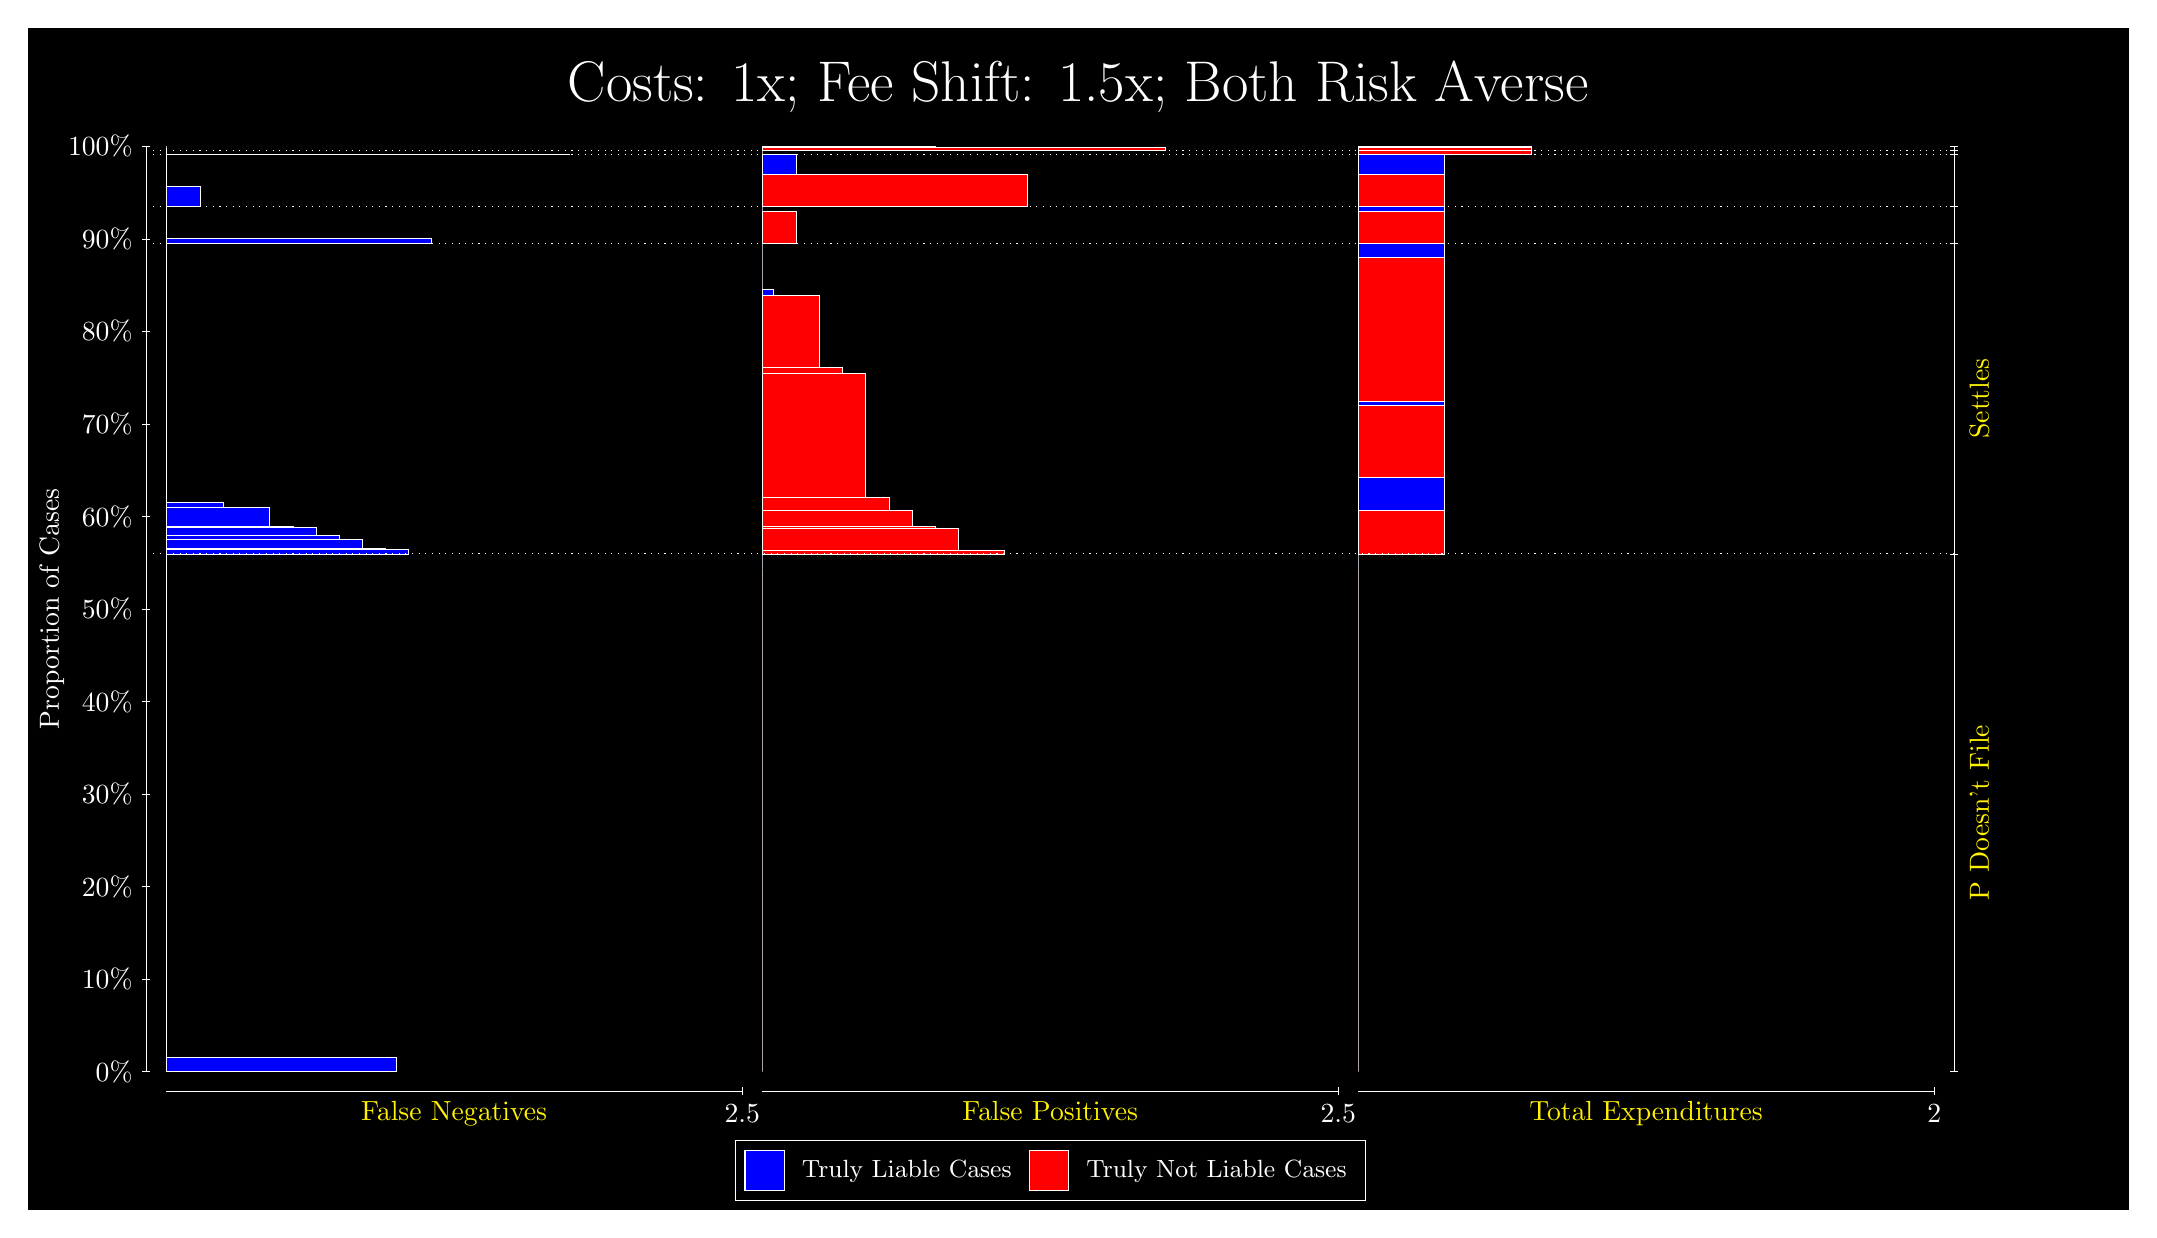
\begin{tikzpicture}
\draw[fill=black] (0,0) rectangle (26.667,15);
\draw[text=white] (0,13.5) rectangle (26.667,15) node[midway] {\huge Costs: 1x; Fee Shift: 1.5x; Both Risk Averse};
\draw[white, very thin] (1.5,1.75) -- (1.5,13.5);
\node[rotate=90, text=white, anchor=center] at (0.3, 7.625) {Proportion of Cases};
\draw[white, very thin] (1.45,1.75) -- (1.55,1.75);
\node[text=white, anchor=east] at (1.45, 1.75) {0\%};
\draw[white, very thin] (1.45,2.925) -- (1.55,2.925);
\node[text=white, anchor=east] at (1.45, 2.925) {10\%};
\draw[white, very thin] (1.45,4.1) -- (1.55,4.1);
\node[text=white, anchor=east] at (1.45, 4.1) {20\%};
\draw[white, very thin] (1.45,5.275) -- (1.55,5.275);
\node[text=white, anchor=east] at (1.45, 5.275) {30\%};
\draw[white, very thin] (1.45,6.45) -- (1.55,6.45);
\node[text=white, anchor=east] at (1.45, 6.45) {40\%};
\draw[white, very thin] (1.45,7.625) -- (1.55,7.625);
\node[text=white, anchor=east] at (1.45, 7.625) {50\%};
\draw[white, very thin] (1.45,8.8) -- (1.55,8.8);
\node[text=white, anchor=east] at (1.45, 8.8) {60\%};
\draw[white, very thin] (1.45,9.975) -- (1.55,9.975);
\node[text=white, anchor=east] at (1.45, 9.975) {70\%};
\draw[white, very thin] (1.45,11.15) -- (1.55,11.15);
\node[text=white, anchor=east] at (1.45, 11.15) {80\%};
\draw[white, very thin] (1.45,12.325) -- (1.55,12.325);
\node[text=white, anchor=east] at (1.45, 12.325) {90\%};
\draw[white, very thin] (1.45,13.5) -- (1.55,13.5);
\node[text=white, anchor=east] at (1.45, 13.5) {100\%};

\draw[white, very thin] (24.457,1.75) -- (24.457,13.5);
\draw[white, very thin] (24.407,1.75) -- (24.507,1.75);
\node[anchor=west] at (24.407, 1.75) {};
\draw[white, very thin] (24.407,8.3248) -- (24.507,8.3248);
\node[anchor=west] at (24.407, 8.3248) {};
\draw[white, very thin] (24.407,12.268) -- (24.507,12.268);
\node[anchor=west] at (24.407, 12.268) {};
\draw[white, very thin] (24.407,12.733) -- (24.507,12.733);
\node[anchor=west] at (24.407, 12.733) {};
\draw[white, very thin] (24.407,13.401) -- (24.507,13.401);
\node[anchor=west] at (24.407, 13.401) {};
\draw[white, very thin] (24.407,13.452) -- (24.507,13.452);
\node[anchor=west] at (24.407, 13.452) {};
\draw[white, very thin] (24.407,13.5) -- (24.507,13.5);
\node[anchor=west] at (24.407, 13.5) {};

\draw[white, very thin, fill=blue] (1.75,1.75) rectangle (4.6775,1.9338);
\draw[white, very thin, fill=red] (1.75,1.9338) rectangle (1.75,8.3248);
\draw[white, very thin, fill=blue] (1.75,8.3248) rectangle (4.8239,8.3808);
\draw[white, very thin, fill=blue] (1.75,8.3808) rectangle (4.5312,8.3961);
\draw[white, very thin, fill=blue] (1.75,8.3961) rectangle (4.2384,8.5038);
\draw[white, very thin, fill=blue] (1.75,8.5038) rectangle (3.9457,8.5637);
\draw[white, very thin, fill=blue] (1.75,8.5637) rectangle (3.6529,8.6669);
\draw[white, very thin, fill=blue] (1.75,8.6669) rectangle (3.3602,8.6778);
\draw[white, very thin, fill=blue] (1.75,8.6778) rectangle (3.0674,8.9137);
\draw[white, very thin, fill=blue] (1.75,8.9137) rectangle (2.4819,8.9793);
\draw[white, very thin, fill=red] (1.75,8.9793) rectangle (1.75,12.268);
\draw[white, very thin, fill=blue] (1.75,12.268) rectangle (5.1167,12.33);
\draw[white, very thin, fill=red] (1.75,12.33) rectangle (1.75,12.733);
\draw[white, very thin, fill=blue] (1.75,12.733) rectangle (2.1891,12.992);
\draw[white, very thin, fill=red] (1.75,12.992) rectangle (1.75,13.401);
\draw[white, very thin, fill=blue] (1.75,13.401) rectangle (6.8732,13.405);
\draw[white, very thin, fill=red] (1.75,13.405) rectangle (1.75,13.452);
\draw[white, very thin, fill=red] (1.75,13.452) rectangle (1.75,13.488);
\draw[white, very thin, fill=blue] (1.75,13.488) rectangle (1.75,13.5);
\draw[white, very thin, fill=red] (9.3189,1.75) rectangle (9.3189,8.141);
\draw[white, very thin, fill=blue] (9.3189,8.141) rectangle (9.3189,8.3248);
\draw[white, very thin, fill=red] (9.3189,8.3248) rectangle (12.393,8.375);
\draw[white, very thin, fill=red] (9.3189,8.375) rectangle (11.807,8.6494);
\draw[white, very thin, fill=red] (9.3189,8.6494) rectangle (11.515,8.6742);
\draw[white, very thin, fill=red] (9.3189,8.6742) rectangle (11.222,8.8791);
\draw[white, very thin, fill=red] (9.3189,8.8791) rectangle (10.929,9.0428);
\draw[white, very thin, fill=red] (9.3189,9.0428) rectangle (10.636,10.614);
\draw[white, very thin, fill=red] (9.3189,10.614) rectangle (10.344,10.697);
\draw[white, very thin, fill=red] (9.3189,10.697) rectangle (10.051,11.614);
\draw[white, very thin, fill=blue] (9.3189,11.614) rectangle (9.4652,11.679);
\draw[white, very thin, fill=blue] (9.3189,11.679) rectangle (9.3189,12.268);
\draw[white, very thin, fill=red] (9.3189,12.268) rectangle (9.758,12.671);
\draw[white, very thin, fill=blue] (9.3189,12.671) rectangle (9.3189,12.733);
\draw[white, very thin, fill=red] (9.3189,12.733) rectangle (12.686,13.143);
\draw[white, very thin, fill=blue] (9.3189,13.143) rectangle (9.758,13.401);
\draw[white, very thin, fill=red] (9.3189,13.401) rectangle (9.3189,13.448);
\draw[white, very thin, fill=blue] (9.3189,13.448) rectangle (9.3189,13.452);
\draw[white, very thin, fill=red] (9.3189,13.452) rectangle (14.442,13.488);
\draw[white, very thin, fill=blue] (9.3189,13.488) rectangle (11.515,13.5);
\draw[white, very thin, fill=red] (16.888,1.75) rectangle (16.888,8.141);
\draw[white, very thin, fill=blue] (16.888,8.141) rectangle (16.888,8.3248);
\draw[white, very thin, fill=red] (16.888,8.3248) rectangle (17.986,8.8791);
\draw[white, very thin, fill=blue] (16.888,8.8791) rectangle (17.986,9.2947);
\draw[white, very thin, fill=red] (16.888,9.2947) rectangle (17.986,10.212);
\draw[white, very thin, fill=blue] (16.888,10.212) rectangle (17.986,10.268);
\draw[white, very thin, fill=red] (16.888,10.268) rectangle (17.986,12.085);
\draw[white, very thin, fill=blue] (16.888,12.085) rectangle (17.986,12.268);
\draw[white, very thin, fill=red] (16.888,12.268) rectangle (17.986,12.671);
\draw[white, very thin, fill=blue] (16.888,12.671) rectangle (17.986,12.733);
\draw[white, very thin, fill=red] (16.888,12.733) rectangle (17.986,13.143);
\draw[white, very thin, fill=blue] (16.888,13.143) rectangle (17.986,13.401);
\draw[white, very thin, fill=red] (16.888,13.401) rectangle (19.083,13.448);
\draw[white, very thin, fill=blue] (16.888,13.448) rectangle (19.083,13.452);
\draw[white, very thin, fill=red] (16.888,13.452) rectangle (19.083,13.488);
\draw[white, very thin, fill=blue] (16.888,13.488) rectangle (19.083,13.5);
\draw[white, dotted] (1.5,8.3248) -- (24.457,8.3248);
\draw[white, dotted] (1.5,12.268) -- (24.457,12.268);
\draw[white, dotted] (1.5,12.733) -- (24.457,12.733);
\draw[white, dotted] (1.5,13.401) -- (24.457,13.401);
\draw[white, dotted] (1.5,13.452) -- (24.457,13.452);
\draw[white, very thin] (1.75,1.5) -- (9.0689,1.5);
\node[text=yellow, anchor=north] at (5.4094, 1.5) {False Negatives};
\draw[white, very thin] (9.0689,1.45) -- (9.0689,1.55);
\node[text=white, anchor=north] at (9.0689, 1.45) {2.5};

\draw[white, very thin] (9.3189,1.5) -- (16.638,1.5);
\node[text=yellow, anchor=north] at (12.978, 1.5) {False Positives};
\draw[white, very thin] (16.638,1.45) -- (16.638,1.55);
\node[text=white, anchor=north] at (16.638, 1.45) {2.5};

\draw[white, very thin] (16.888,1.5) -- (24.207,1.5);
\node[text=yellow, anchor=north] at (20.547, 1.5) {Total Expenditures};
\draw[white, very thin] (24.207,1.45) -- (24.207,1.55);
\node[text=white, anchor=north] at (24.207, 1.45) {2};

\node[text=yellow, centered, rotate=90] at (24.777, 5.0374) {P Doesn't File};
\node[text=yellow, centered, rotate=90] at (24.777, 10.297) {Settles};





\draw (12.978300999999998,1.5) node[draw=none] (baseCoordinate) {};
\begin{scope}[align=center]
        \matrix[scale=0.5, draw=white, below=0.5cm of baseCoordinate, nodes={draw}, column sep=0.1cm]{
            \node[rectangle, draw, minimum width=0.5cm, minimum height=0.5cm, fill=blue] {}; &
            \node[draw=none, font=\small, text=white] (B) {Truly Liable Cases}; &
            \node[rectangle, draw, minimum width=0.5cm, minimum height=0.5cm, fill=red] {}; &
            \node[draw=none, font=\small, text=white] (B) {Truly Not Liable Cases}; \\
            };
\end{scope}

\end{tikzpicture}
\end{document}